%-----------------------------------------------%
%---------------------------------------------%
%
% BACHELOR OF SCIENCE THESIS ~ SLIDES
%
% Emanuele Ballarin <emanuele@ballarin.cc>
%
% Prof. Luca Bortolussi, Prof. Fabio Benatti
%
%---------------------------------------------%
%
% Bachelor's Degree in Physics
%
% Dept. of Physics
% University of Trieste, Italy
%
% 24-27/04/2020
%
% A.Y. 2018/2019
%
%
% Authored on 20/04/2020
%
%
%---------------------------------------------%
%-----------------------------------------------%



\documentclass{beamer}

\usepackage[utf8]{inputenc}
\usepackage[italian]{babel}

\usepackage{graphicx}
\usepackage{amsmath}
\usepackage{mathtools}
\usepackage{wrapfig}
\usepackage{amsfonts}
\usepackage{csquotes}
\usepackage{epigraph}
\usepackage{float}
\usepackage{lipsum}
\usepackage{blindtext}
\usepackage{multirow}
\usepackage[ruled,vlined]{algorithm2e}
\usepackage{bm}
\usepackage{xcolor}
\usepackage{upgreek}
\usepackage{calc}
\usepackage{lscape}

% TYPESETTING SUGAR
\DeclareMathOperator*{\argmax}{argmax}
\DeclareMathOperator*{\argmin}{argmin}
\DeclareMathOperator*{\Find}{Find}
\DeclareMathOperator*{\find}{find}
\DeclareMathOperator*{\NNet}{NNet}
\DeclareMathOperator*{\EGR}{EGR}
\def\leq{\leqslant}
\def\geq{\geqslant}

\usetheme{Madrid}

%-----------------------------------------------%
%-----------------------------------------------%



%
% TITLE SLIDE
%

\title [Reti neurali, robustezza, modelli generativi] {Modelli generativi di modelli neurali artificiali robusti}
\subtitle{Uno studio preliminare di fattibilità}

\author[E. Ballarin] {Emanuele \textsc{Ballarin}\inst{$\dagger$}\\[2.9mm]% Vertical space is fixed; Horizontal space is tailored for names
	{\small Relatore: \hspace{2.5mm}Prof. Luca \textsc{Bortolussi}\inst{$\ddagger$} \\ Co-Relatore: Prof. Fabio \textsc{Benatti}\inst{$\dagger$}\inst{$\diamond$}}}

\institute[Dip. di Fisica, Univ. di Trieste]
{
	\inst{$\dagger$}
	Dipartimento di Fisica, Univ. di Trieste\\
	\inst{$\ddagger$}
	Dipartimento di Matematica e Geoscienze, Univ. di Trieste\\
	\inst{$\diamond$}
	INFN, sezione di Trieste
}

\date[Sess. di Laurea del 24/04/2020]
{Sessione di Laurea straordinaria -- 24 aprile 2020}

\titlegraphic{
\includegraphics[width=1.25cm,height=1.3cm,keepaspectratio]{dssclogo.png}
	\hspace*{93.04mm}~% Horizontal space is tailored for 1.3cm square logos
	
\includegraphics[width=1.3cm,height=1.25cm,keepaspectratio]{logouniv.png}
}

%-----------------------------------------------%
%-----------------------------------------------%



%
% ADAPTIVE TABLE OF CONTENTS
%

\AtBeginSection[]
{
	\begin{frame}
		\frametitle{\textit{Voi siete qui}}
		\tableofcontents[currentsection]
	\end{frame}
}

%-----------------------------------------------%
%-----------------------------------------------%



%
% DOCUMENT
%

\begin{document}

% Insert title slide
\frame{\titlepage}

%-----------------------------------------------%


%% INTRODUZIONE AL DEEP LEARNING

\section{Introduzione al paradigma del \textit{Deep Learning}}{

%% SLIDE 1.1:
\begin{frame}
\frametitle{\textit{Deep Learning} $\subseteq$ \textit{Machine Learning}}
	%-----------------------------------------%
	Il \textit{Machine Learning} è essenzialmente studio e implementazione di \textbf{\textit{algoritmi d'apprendimento}}. In particolare: apprendimento \textit{statistico}.

	\hfill\break

	\begin{displayquote}
		\textit{``Un programma informatico impara da un'esperienza $E$ con riferimento ad un'attività $T$ e una misura di prestazioni $P$ se le sue prestazioni misurate da $P$ nello svolgimento dell'attività $T$ migliorano noto $E$.”}\\
		{\raggedleft(Mitchell, 1998)\par}
	\end{displayquote}

	\hfill\break

	\begin{block}{Nota}
			Più che \textit{un} algoritmo, il \textit{Deep Learning} è un approccio paradigmatico e \alert{universale} alla risoluzione di problemi d'\textit{apprendimento automatico}.
	\end{block}
	%-----------------------------------------%
\end{frame}

%---------------------------------------------%

%% SLIDE 1.2:
\begin{frame}
	\frametitle{I problemi di \textit{classificazione} automatica (\textit{supervisionata})}
	%-----------------------------------------%
	Spazio degli \textit{input}: $\mathbb{I} \sim \mathbb{R}^{k}$ -- Ciò che si vuole classificare\\
	Spazio degli \textit{output} (o \textit{delle classi}): $\mathbb{O}$ -- Classi in cui \textbf{partizionare} $\mathbb{I}$\\

	\hfill\break

	\textit{Training set}: $\{\mathbb{I}\times\mathbb{O}\} \supseteq \mathcal{T} = \{(\boldsymbol{x}_1, \xi_1), (\boldsymbol{x}_2, \xi_2), \ \dots,\ (\boldsymbol{x}_n, \xi_n)\}$ -- Esempi

	\hfill\break

	Un classificatore $\mathcal{C}_{\boldsymbol{w}, \boldsymbol{h}}: \ \mathbb{I} \rightarrow \mathbb{O}$ dipende da \textbf{pesi} ($\boldsymbol{w}$) e \textbf{iperparametri} ($\boldsymbol{h}$).

	%\hfill\break

	\textit{Loss function}: $\mathcal{L} = \mathcal{L}(\mathcal{C}_{\boldsymbol{w}, \boldsymbol{h}}, \mathcal{T})$

	\hfill\break

	Scopo del \textit{training}: trovare $\boldsymbol{w}$ ottimale per $\mathcal{C}$, noti $\mathcal{T}, \boldsymbol{h}, \mathcal{L}$


	\begin{block}{Questo è equivalente al problema di \alert{ottimizzazione}:}
		$$\Find \boldsymbol{\tilde{w}} = \argmin_{\boldsymbol{w}}\left(\mathcal{L}\left(\mathcal{C}_{\boldsymbol{w}, \boldsymbol{h}}, \mathcal{T}\right)\right)$$
	\end{block}
	%-----------------------------------------%
\end{frame}

%---------------------------------------------%

%% SLIDE 1.3:
\begin{frame}
	\frametitle{Il \textit{Perceptron} \textit{(Rosenblatt, 1958)}}

	Il \textit{Perceptron} è un modello che opera sugli \textit{input} con una \textbf{trasformazione affine} seguita da una \alert{\textit{non-linearità}} ($A$)

	$$
	y = A \left( \boldsymbol{x} \cdot \boldsymbol{w} + b \right) = A \left( \sum_{j=1}^{k}{x_j w_j + b} \right)
	$$

	e dotato di un semplice \textit{training step} iterativo:

	$$
	\boldsymbol{w'} \leftarrow \left( \boldsymbol{w} + \epsilon \left( \xi_i - y_i \right) \boldsymbol{x}_i  \right)
	$$
	$$
	b' \leftarrow \left( b + \epsilon \left( \xi_i - y_i \right) \right)
	$$

	\begin{alertblock}{Nota}
		Il \textit{Perceptron} non è solo un \textit{classificatore}. È però in grado di risolvere solo una ristretta classe di problemi. \textit{(Minsky \& Papert, 1696)}
	\end{alertblock}

\end{frame}

%---------------------------------------------%

%% SLIDE 1.3bis:
\begin{frame}
	\frametitle{Il \textit{Perceptron} (Rosenblatt, 1958) [cont.]}
		\center 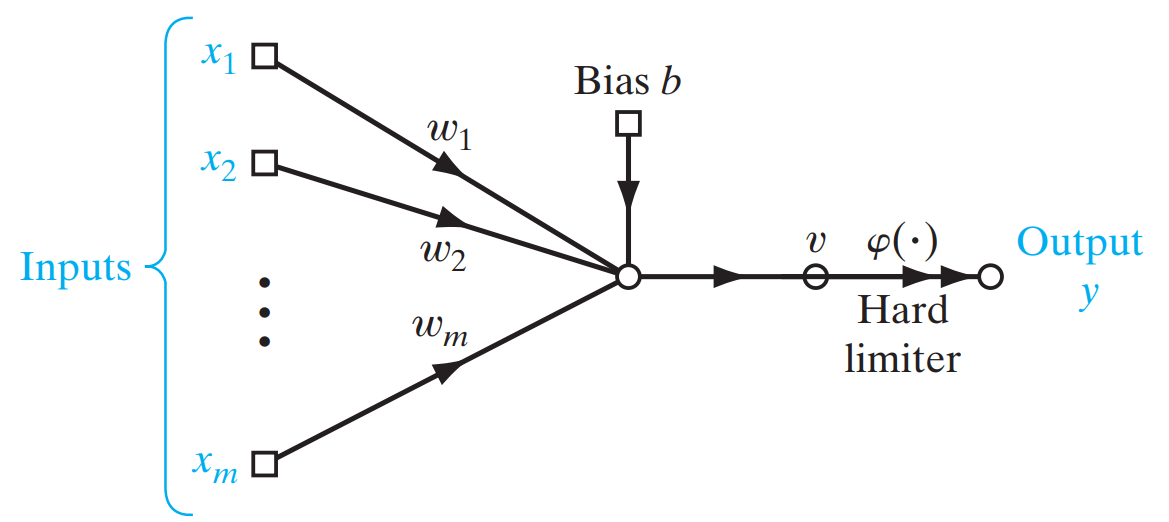
\includegraphics[height=5cm, keepaspectratio]{perceptron.png}
\end{frame}

%---------------------------------------------%

%% SLIDE 1.4:
\begin{frame}
	\frametitle{\textit{Going deeper}}
		\begin{block}{What if$\dots$?}
			E se un problema d'apprendimento (arbitrario) fosse sempre \textbf{scomponibile} in sottoproblemi \textit{perceptron-separabili}?
	\end{block}
	\center 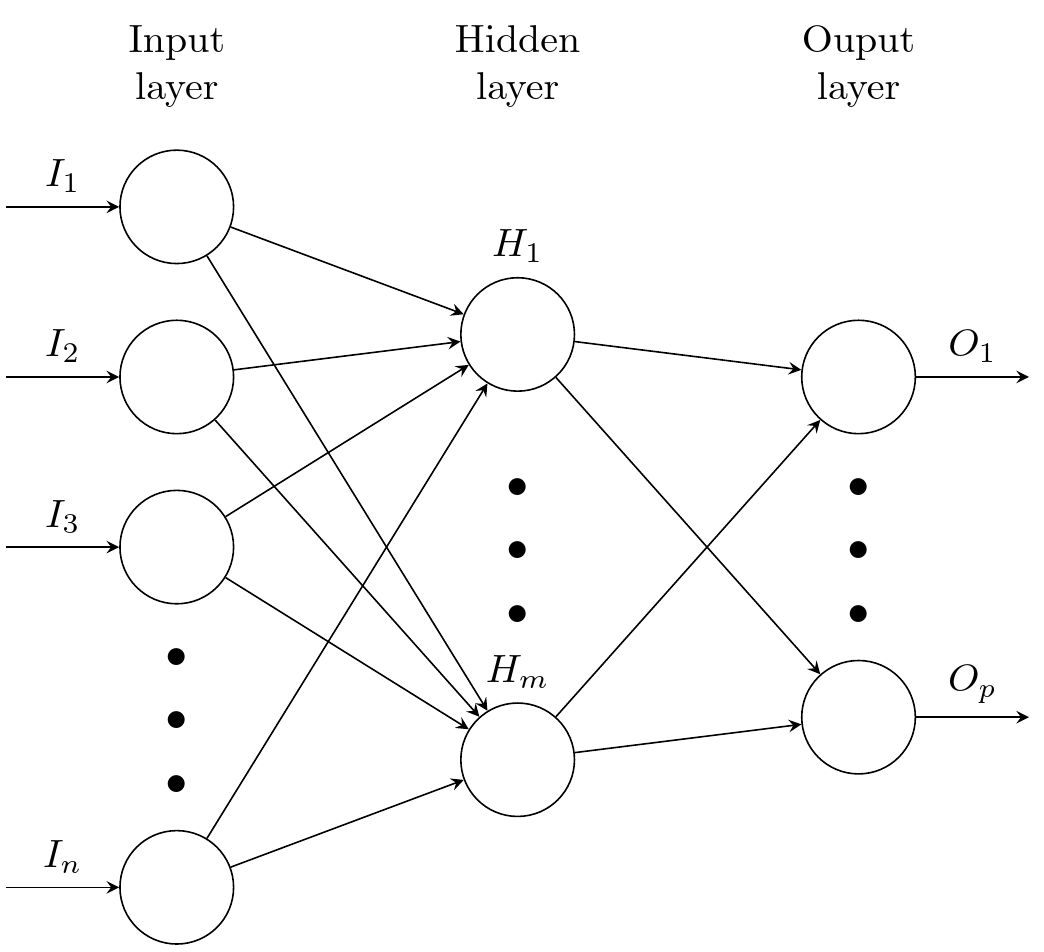
\includegraphics[width=0.55\linewidth]{nnet-graph.png}
\end{frame}

%---------------------------------------------%

%% SLIDE 1.4bis:
\begin{frame}
	\frametitle{\textit{Going deeper} [cont.]}

	Questo introduce una classe di modelli assai più \textit{espressivi} e \textit{capaci}: i \textit{fully-connected multilayer perceptron models}.

	\hfill\break

	E il concetto di \alert{\textit{layer}}

	$$
	L_r(\boldsymbol{x}_r) = A_r\left(  \boldsymbol{W}_r \boldsymbol{x}_r + \boldsymbol{b}_r \right)
	$$.

	\hfill\break

	Un'intera rete neurale può essere descritta come:

	$$
	\boldsymbol{y} = \NNet(\boldsymbol{x}) = L_N( L_{N-1}(\dots (L_1(\boldsymbol{x}))) )
	$$.

\end{frame}

%---------------------------------------------%

%% SLIDE 1.5:
\begin{frame}
	\frametitle{\textit{Going deeper} [cont.]}
	Il problema d'ottimizzazione diventa però \alert{intrattabile} con tecniche tradizionali. Si estende quindi l'approccio iterativo: \textit{gradient descent}.

	$$
	\boldsymbol{\theta'} \leftarrow \boldsymbol{\theta} - \epsilon \boldsymbol{g}
	$$
	(con $\boldsymbol{\theta}$ vettore dei pesi del modello, $\boldsymbol{g} = \nabla_{\boldsymbol{\theta}}\mathcal{L}$, $\epsilon \ll 1$)

	\hfill\break

	O sue varianti più efficaci (\textit{g.d. with $1^{\text{st}}$ momentum correction}):
	$$
	\boldsymbol{v}_t \leftarrow \boldsymbol{\theta}_t - \boldsymbol{\theta}_{t-1}
	$$
	$$
	\boldsymbol{\theta}_{t+1} \leftarrow \boldsymbol{\theta}_{t} - \epsilon \boldsymbol{g}_{t} + \mu \boldsymbol{v}_t
	$$
	(con $t$ l'indice di iterazione, $\mu \ll 1$)
\end{frame}

%---------------------------------------------%

%% SLIDE 1.4:
\begin{frame}
	\frametitle{\textit{Going deeper} [cont.]}
	\center 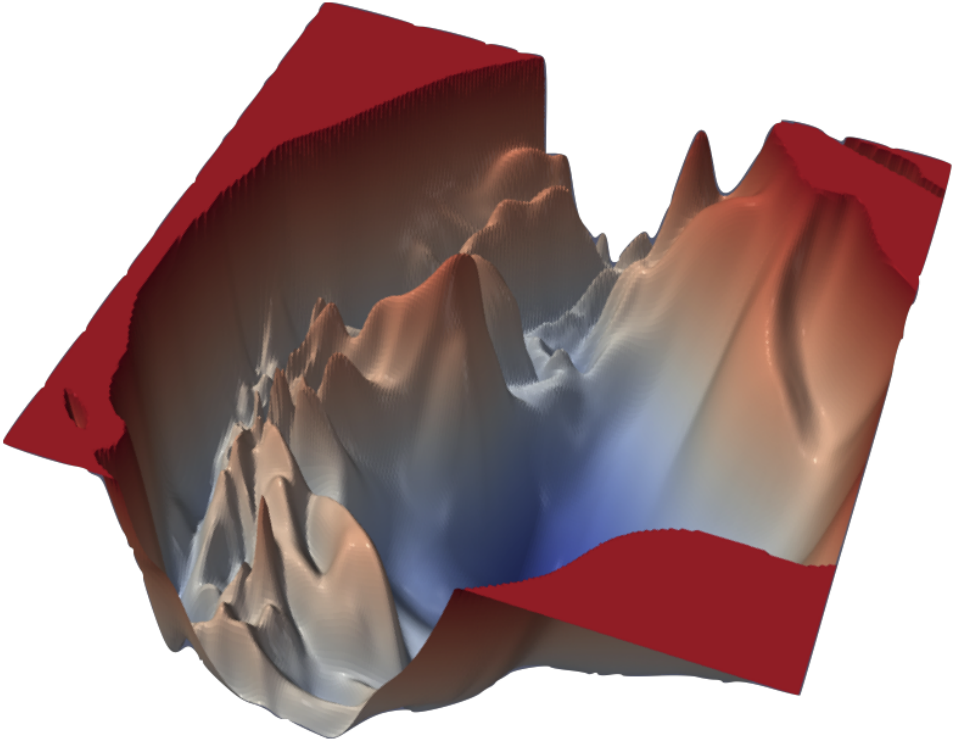
\includegraphics[width=0.8\linewidth]{loss-landscape.png}
\end{frame}

%---------------------------------------------%

%% SLIDE 1.5:
\begin{frame}
	\frametitle{I risultati del \textit{Deep Learning}}
	Il \textit{Deep Learning} è un paradigma maturo, capace di risultati tutt'ora ineguagliati in problemi di \textit{regressione predittiva}, \textit{classificazione}, \textit{generazione} di dati, \textit{controllo}.

	\hfill\break

		\center 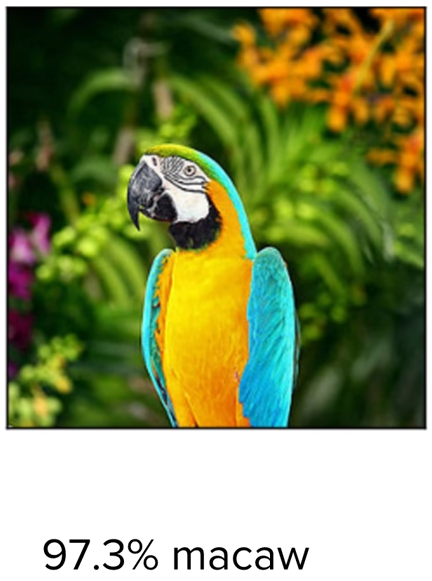
\includegraphics[height=0.35\linewidth]{pappagallo.png}



\end{frame}

%---------------------------------------------%

%% SLIDE 1.6:
\begin{frame}
	\frametitle{\textit{Tutto chiaro?}}
	Forse no.

	\hfill\break

	\center 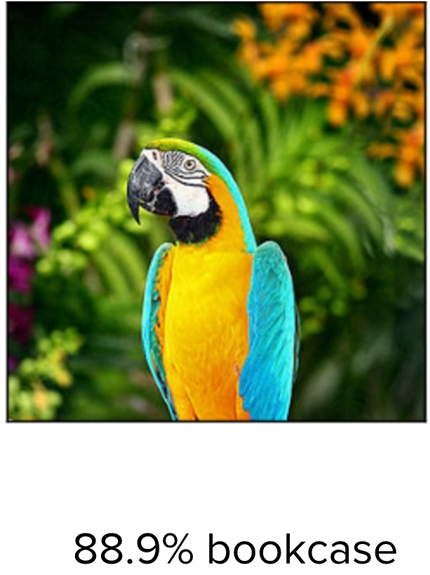
\includegraphics[height=0.35\linewidth]{libreria.png}

	\hfill\break
	\center{\textit{(stesso classificatore; immagine \alert{quasi} identica)}}
\end{frame}

}

%-----------------------------------------------%


%% LA ROBUSTEZZA

\section{Il problema della \textit{robustezza}}{

%% SLIDE 2.1:
\begin{frame}
	\frametitle{Perché studiare la \textit{robustezza}?}
	Il fenomeno appena mostrato (\textit{Perdikaris, 2018}) è un esempio di \textit{assenza di \alert{robustezza}} nel classificatore utilizzato.
	\hfill\break

	Lo studio di questi fenomeni si presta ad analizzare:
	\hfill\break

	\begin{itemize}
		\item{La validità del classificatore in scenari di \textbf{difficile prevedibilità}, rari, inusuali;}
		\item{La resistenza del classificatore a manipolazioni \textbf{dolose} degli \textit{input}};
	\end{itemize}
	\hfill\break
	E di adottare eventuali mitigazioni.

	\hfill\break

	Ma cosa provoca questo tipo di comportamenti?
\end{frame}

%---------------------------------------------%

%% SLIDE 2.2:
\begin{frame}
	\frametitle{La \textit{Manifold Hypothesis} \textit{(Dube, 2018)}}
	Un'ipotesi da tempo circolante all'interno della comunità dei ricercatori, ma solo recentemente associata ai fenomeni di \textit{robustezza}.
	\hfill\break

	\begin{itemize}
		\item{Un classificatore (anche non \textit{neurale}) accetta \textbf{qualsiasi} \textit{input} compatibile con la codifica scelta.}
		\item{Il contenuto del \textit{training set} descrive una varietà \textit{\textbf{basso}-dimensionale} immersa in un \textit{input space} \textit{\textbf{alto}-dimensionale}.\\Ciò resta vero anche per le \textit{\alert{decision boundaries}} apprese.}
		\item{Lo scopo del \textit{training} è quello di apprendere le \textbf{intersezioni} tra \textit{data manifold} e \textit{decision boundaries};}
	\end{itemize}
\end{frame}

%---------------------------------------------%

%% SLIDE 2.3:
\begin{frame}
	\frametitle{\textit{Adversarial attacks}}
	Un \textit{adversarial attack} è una procedura (o il suo risultato) atta a provocare un comportamento \alert{non previsto} o \alert{non voluto} in un classificatore -- cioè a produrre una \textit{misclassification}.

	\hfill\break

	Due approcci:

	\begin{itemize}
	\item{\textbf{Perturbazioni} da \textit{input} d'interesse (esempio precedente);}
	\item{\textit{Input} privi di significato noto (vedi sotto).}
	\end{itemize}

	\center{ 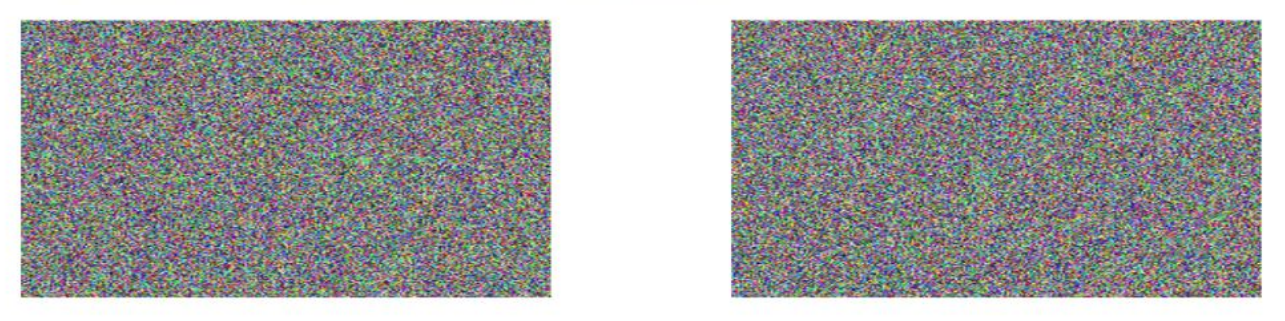
\includegraphics[height=0.2\linewidth]{fake-tajmahal.png}}\\
	{\raggedleft(\textit{Taj Mahal; $\sim 65\%$})\par}

\end{frame}

%---------------------------------------------%

%% SLIDE 2.4:
\begin{frame}
	\frametitle{Misure di \textit{robustezza perturbativa}}
	Il \textit{caso perturbativo} è sicuramente quello più simile a \textit{input} imprevisti raccolti in uno scenario realistico o a causa di manomissioni.
	\hfill\break

	\begin{block}{\textit{$\epsilon$-robustezza} -- di $\mathcal{C}$, in $\boldsymbol{x} \in \mathbb{I}$, rispetto a $||\cdot||$}
		$$
		\forall \boldsymbol{p} \ \text{t.c.} \ ||\boldsymbol{p}|| < \alert{\epsilon}, \ \mathcal{C}(\boldsymbol{x}) \alert{=} \mathcal{C}(\boldsymbol{x} +\boldsymbol{p} )
		$$
	\end{block}

	\begin{block}{\textit{Empirical Global Robustness} -- di $\mathcal{C}$, dati $\mathcal{\tilde{T}} \subseteq \mathcal{T}$ e un \textit{attacco}}
		$$\EGR({\tilde{\mathcal{T}}}) = \left( 1 - \frac{\# \text{(attacks leading to misclassification)}}{|\mathcal{\tilde{T}}|} \right)$$
	\end{block}

\end{frame}

%---------------------------------------------%

%% SLIDE 2.5:
\begin{frame}
	\frametitle{Esempio di attacco: \textit{PGD-${||\cdot||}_{\infty}$}}

	È un attacco \textit{white-box}: richiede \textbf{completa} conoscenza del modello $\mathcal{C}$ e della sua \textit{loss} $\mathcal{L}$.
	\hfill\break

	Dato $\tilde{\boldsymbol{x}} \in \mathbb{I}$ di corretta classificazione e fissato $\alert{\epsilon}$, \textbf{iterativamente}:
	\begin{enumerate}
		\item {Ci si pone in $\tilde{\boldsymbol{x}}$ o in qualunque altro punto della palla chiusa $\mathcal{B}_{\alert{\epsilon}}{(\tilde{\boldsymbol{x}})}$ };
		\item { Si effettua un \textit{update step}: $\boldsymbol{x'} \leftarrow \boldsymbol{x} + {\eta} \nabla_{\boldsymbol{x}}\mathcal{L}\left(\mathcal{C}_{\boldsymbol{w}, \boldsymbol{h}}{\left({\boldsymbol{x}}\right)}\right)$; $\eta \ll 1$ };
		\item{ Qualora $\boldsymbol{x'}$ $\notin$  $\mathcal{B}_{{\epsilon}}{(\tilde{\boldsymbol{x}})}$, lo si proietta sulla sfera $\mathcal{S}_{{\epsilon}}{(\tilde{\boldsymbol{x}})}$ }.
	\end{enumerate}




	\begin{block}{È equivalente al problema di ottimizzazione:}
		$$\Find \boldsymbol{x}' = \argmin_{\alert{\boldsymbol{x}} \in \mathcal{B}_{\alert{\epsilon}}{(\tilde{\boldsymbol{x}})}}\left(-\mathcal{L}\left(\mathcal{C}_{\boldsymbol{w}, \boldsymbol{h}}{\left(\alert{\boldsymbol{x}}\right)}\right)\right)$$
	\end{block}
\hfill\break
Le metriche scelte devono essere quelle indotte da ${||\cdot||}_{\infty}$.
\end{frame}

%---------------------------------------------%

%% SLIDE 2.5bis:
\begin{frame}
	\frametitle{Esempio di attacco: \textit{PGD-${||\cdot||}_{\infty}$} [esempio nel caso ${||\cdot||}_{2}$]}
	\center 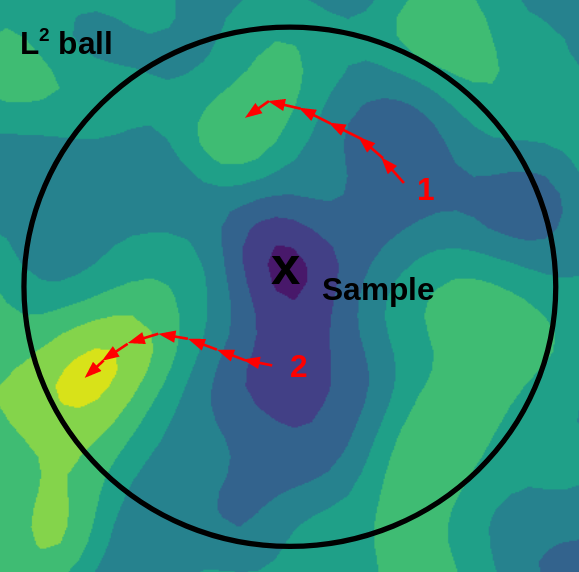
\includegraphics[height=0.60\linewidth]{pgdball.png}
\end{frame}

%---------------------------------------------%

%% SLIDE 2.6:
\begin{frame}
	\frametitle{Difese e \textit{adversarial training}}
	In generale sono stati proposti numerosi \textit{attacchi} per sistemi di \textit{Deep Learning}. Così come per gli \textit{attacchi} sono state proposte altrettante \textit{difese}. Si cerca (e spesso si ottiene) la \textbf{trasferibilità}.

	\hfill\break
	Un principio molto popolare è quello dell'\textit{adversarial training}: proseguire l'allenamento su un \textit{training set} contenente i risultati di \textit{attacchi} generati allo scopo.

	\hfill\break
	\begin{alertblock}{Nota}
		In generale, tuttavia, non sembra mai essere messo in discussione il meccanismo con cui i \textit{pesi} debbano essere generati: tramite \textit{gradient descent} \alert{sul modello stesso}.
	\end{alertblock}
\end{frame}

}

%-----------------------------------------------%


%% LA NOSTRA PROPOSTA

\section{La nostra proposta}{

%% SLIDE 3.1:
\begin{frame}
	\frametitle{Modelli generativi dei pesi}
	\begin{displayquote}
		\textit{``Nessuna metodologia di difesa contro \textit{adversarial examples} è tuttavia completamente soddisfacente. Questo rimane un campo di ricerca aperto e in rapida evoluzione.”}\\
		{\raggedleft(Kurakin, Goodfellow \& Bengio, 2018)\par}
	\end{displayquote}

\hfill\break

\begin{block}{L'idea}
	Apprendere un modello (accompagnato da un'opportuno \textit{protocollo di training}) con lo scopo di \alert{generare \textit{pesi} di architetture neurali} di forma prestabilita.
\end{block}




\end{frame}

%---------------------------------------------%

%% SLIDE 3.2:
\begin{frame}
	\frametitle{Generatore $\mathcal{G}$ e \textit{value network} $\mathcal{V}$}
	Un riassunto della dinamica di \textit{training}:
	\hfill\break

	\begin{enumerate}
		\item \textbf{Campionamento}: $\boldsymbol{s} \sim \text{Dist}^{z}$ nota;
		\item Generazione dei pesi:  $\boldsymbol{\theta} = \mathcal{G}(\boldsymbol{s})$ e \textit{weight-loading};
		\item Computo di \textit{accuratezza} $\mathfrak{A}$ e \textit{robustezza} $\mathfrak{R}$ su $\tilde{T} \subseteq \mathcal{T}$;
		\item \textbf{Stima} di \textit{accuratezza} e \textit{robustezza} tramite $(\hat{\mathfrak{A}},\hat{\mathfrak{R}}) = \mathcal{V}(\boldsymbol{\theta})$;
		\item \textit{Training step} per $\mathcal{V}$: $\mathcal{L}_{\mathcal{V}} = $ similarità tra $(\hat{\mathfrak{A}},\hat{\mathfrak{R}})$ e $({\mathfrak{A}},{\mathfrak{R}})$
		\item \textit{Training step} $\mathcal{G}$: $\mathcal{L}(\boldsymbol{\theta}) =  -\alpha \alert{\hat{\mathfrak{A}}}(\boldsymbol{\theta}) - \beta \alert{\hat{\mathfrak{R}}}(\boldsymbol{\theta}) \ \text{t.c.}\ \alpha + \beta = 1$.
	\end{enumerate}
\end{frame}

%---------------------------------------------%

%% SLIDE 3.3:
\begin{frame}
	\frametitle{\textit{Where's the catch?}}
	In fase d'ideazione e sviluppo sono stati incontrati alcuni ostacoli che hanno richiesto soluzioni specifiche:
	\hfill\break

	\begin{itemize}
		\item Non-differenziabilità del \textit{weight-loading} $\rightarrow$ Uso di un \textit{value network} $\mathcal{V}$;
		\item Lentezza nella convergenza (a causa di $\mathcal{V}$ e non solo) $\rightarrow$ \textit{pretraining};
	\end{itemize}
	\hfill\break

	E alcune scelte sofferte ma necessarie:
	\hfill\break

	\begin{itemize}
		\item Volontà di preservare informazioni distribuzionali riguardo ai \textit{pesi} $\rightarrow$ Impossibilità di usare \textit{regolarizzazioni};
	\end{itemize}
	\hfill\break


\end{frame}

}

%-----------------------------------------------%


% ESPERIMENTAZIONI

\section{Esperimentazioni}{

%% SLIDE 4.1:
\begin{frame}
	\frametitle{Il dataset: \textit{MNIST}}
	Raccolta di $10000$ immagini in \textit{bianco e nero}, quadrate, $28 \times 28$ pixel. Rappresentate come vettore binario dei $784$ pixel.
	\hfill\break

	Contiene raffigurazioni delle cifre arabe $0-9$ in diverse grafie manoscritte, con annessa classificazione in base alle intenzioni dello scrivente.
	\hfill\break

	Tipico problema di classificazione: uno standard \textit{de facto} per \textit{toy-problems} in \textit{Machine Learning}. Oggi di facile risoluzione quanto all'accuratezza del modello appreso.
	\hfill\break

	\center 
\includegraphics[height=0.18\linewidth]{mnist-sample-four.png}
\end{frame}

	%---------------------------------------------%

%% SLIDE 4.2:
\begin{frame}
	\frametitle{Classificatore (\textit{LeNet-5}) e attacco (\textit{PGD-${||\cdot||}_{\infty}$)}}
	\textit{LeNet5} (LeCun, Bottou et al.) è un'architettura neurale \textit{convoluzionale} e {fully-connected} pensata appositamente per la classificazione di cifre arabe manoscritte. Nel caso in esame è semplicemente stato ridotto per praticità il numero di \textit{pesi}.
	\hfill\break
	\center 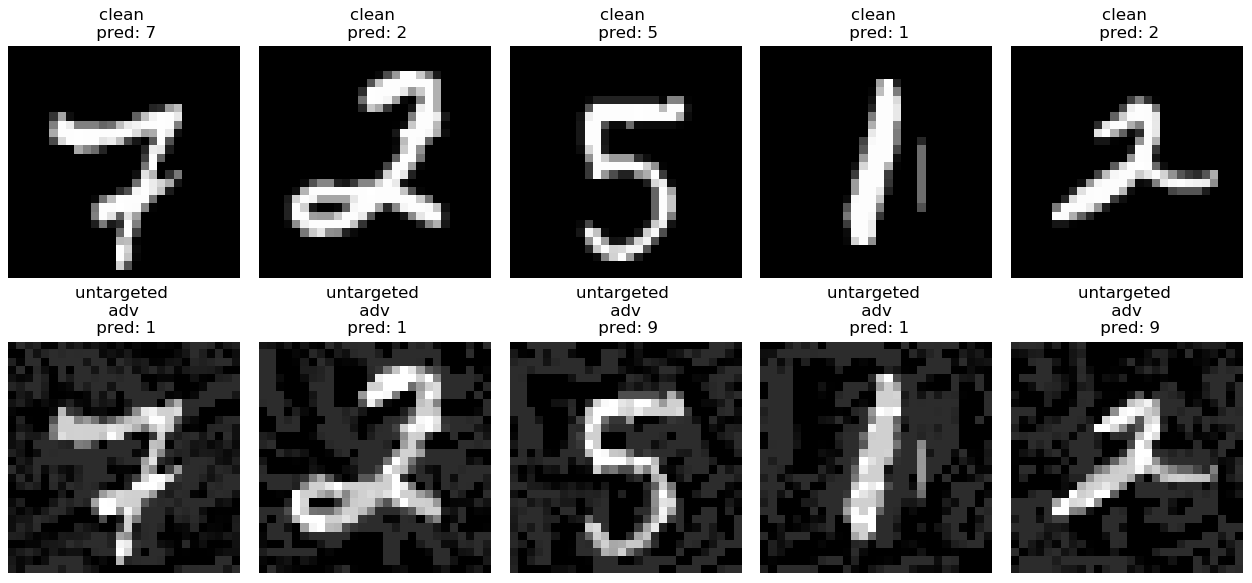
\includegraphics[height=0.40\linewidth]{mnist-adv-pgdlinf.png}
\end{frame}

%---------------------------------------------%

%% SLIDE 4.3:
\begin{frame}
	\frametitle{Risultati}
	Risultati interessanti, seppur fortemente preliminari.
	\hfill\break

	\center 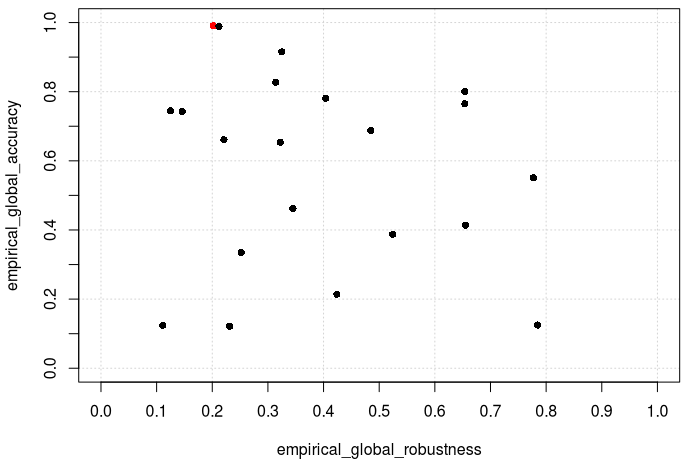
\includegraphics[height=0.58\linewidth]{my-graph-scatterplot.png}

\end{frame}

%---------------------------------------------%

%% SLIDE 4.3:
\begin{frame}
	\frametitle{Conclusioni}
	Alcuni dei risultati evidenziati si configurano come notevoli e interessanti. Il percorso proposto è sicuramente meritevole di ulteriori \alert{approfondimenti}. L'ambito è ancora troppo poco esplorato!

	\hfill\break
	Possibili sviluppi ulteriori:
	\begin{itemize}
		\item{Determinazione delle condizioni rigorose di convergenza del modello;}
		\item{Studio dei campioni con migliore profilo \textit{acc/rob};}
		\item{Ottimizzazione multi-obiettivo nel \textit{latent space};}
		\item{Misure di \textit{acc/rob} differenziabili e ablazione di $\mathcal{V}$;}
		\item{Robustezza \textit{multi-attacco} e \textit{multi-norma};}
	\hfill\break
		\item{Robustezza \textit{weight-agnostic};}
		\item{Approccio \textit{neuro-inspired}/\textit{active learning} alla robustezza;}
	\end{itemize}

\end{frame}

%% THANKS!
\begin{frame}
	\frametitle{Ringraziamenti}
	Grazie per l'attenzione.
\end{frame}

}

%-----------------------------------------------%
%-----------------------------------------------%


\end{document}
